\chapter{Introduction}

\graphicspath{{Chapter1/figures/}}

%The data around the world has been produced more rapidly than ever before. Major sources include sensors, machine logs, public websites and social media. For a single day, 50 million photos are uploaded on Instagram, 500 million tweets are sent on Twitter, 3.5 billion searches are performed on Google and 200 billion emails are sent~\footnote{\url{http://www.internetlivestats.com/}}. Lacking of data is not a problem any more; However it's challenging to understand of make sense of such data.

%https://datafloq.com/read/understanding-sources-big-data-infographic/338\
%http://www.internetlivestats.com/

In a broad context, \emph{sensemaking} reflects how we make sense of the world so that we can take further actions in it~\cite{Snowden2005}. More specifically, sensemaking is described as a motivated and continuous effort to understand the relationships among people, places and events around us in order to act more effectively~\cite{Klein2006a}. It is the process of collecting, organizing and representing complex information sets with an emphasis on some problem we need to solve~\cite{Russell2008}. For example, intelligence analysts may need to examine thousands of reports to establish deep understanding of particular persons or organizations before identifying possible threats from them. In an everyday context such as selecting a smartwatch for purchase, a person may search for different models on the Internet, learn unknown technical terminologies and consider pros and cons between these identified models. Automated techniques in information retrieval and data mining may speed up the sensemaking process. For instance, named-entity recognition technique~\cite{Nadeau2007} can identify and classifies entities in text into predefined categories such as persons, organizations and locations. It saves analysts a considerable amount of time in common tasks such as findings all reports mentioning a particular person. However, human still involves heavily in sensemaking to synthesize knowledge and draw inferences before making informed decisions.

\emph{Visualization} is a computer-based system designed to help people perform tasks more effectively through visual representations of datasets~\cite{Munzner2014}. It can display a large amount of data in a small space and allow for close examination of details through interaction. During the data exploration, many insights, questions and (conflict) hypotheses may appear. Unfortunately, human with limited capacity of working memory cannot simultaneously hold all of these findings. Visualization can help expand working memory by allowing people to externalize internal cognition and memory usage to the visual displays, and organize them in a meaningful structure. For instance, research has shown that spatially grouping of findings and drawing links between them to indicate their relationships can facilitate reasoning and sensemaking~\cite{Sedig2013}.

Not only are the final outcomes of the sensemaking process important, but the process itself is also of great value~\cite{Ragan2016}. \emph{Analytic provenance} captures both the interactive data exploration process and the accompanied human reasoning process during sensemaking~\cite{Xu2015}. This provenance information allows users to recall and revisit the process, typically combining with undo/redo and bookmarking features~\cite{Heer2008}. It also allows reproduction of the process, possibly with a different dataset and parameter settings~\cite{Davidson2007}. Provenance can facilitate learning through building tutorials~\cite{Grabler2009}, presentation~\cite{Eccles2007} and improving communication between teachers and students~\cite{Plaisant1999}. 

Analytic provenance also has the potential to support the on-going sensemaking process, besides many post hoc applications it provides. When a user employs a system to make sense of a problem, her interaction and discovery (both are referred as provenance data) are captured and visualized for providing support back to the sensemaking process. The visualization of provenance data could  provide an overview of the sensemaking process including what has been done, how has it been done, and why has it been done like that. It could show what knowledge the user has learned and offer ways to structure it meaningfully. A through understanding of the past process may guide the user to the next step in making sense of the task. The provenance visualization should be able to communicate with the sensemaking system to facilitate the interplay between the user and these two. \autoref{fig:intro-workflow} illustrates this sensemaking-supporting pipeline. 

\begin{figure}[!htb]
	\centering
	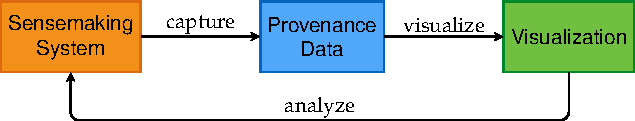
\includegraphics{workflow}
	\caption{A pipeline of supporting sensemaking through analytic provenance. While employing a sensemaking system to solve a task, user interaction and discovery are captured and visualized to provide support back to the sensemaking process.}
	\label{fig:intro-workflow}
\end{figure}

\section{Research Problem and Approach}

\subsection{Problem}
In this thesis, we focus on the \textbf{visualization} part of the sensemaking-supporting pipeline as shown in \autoref{fig:intro-workflow}.
\begin{center}
	\strong{How to design interactive visualizations of provenance data \\for supporting sensemaking?}
\end{center}

%Pirolli and Card~\cite{Pirolli2005} describe sensemaking as a process consisting of two loops: the \emph{foraging loop}, which involves searching, extracting and organizing information; and the \emph{sensemaking loop}, which involves building schemas, generating and testing hypotheses, and presenting the outcome. Schematization plays an important role in this model: connecting the foraging loop and the sensemaking loop. It is a crucial step in converting raw evidence to rational explanations. Pirolli and Card suggest that the schematization process should be supported by a computer-based tool that organizes raw evidence into small-scale stories about typical topics or in answer to typical questions (e.g., who, what, when, where, why, how). This suggestion is aligned with a recent empirical study by Kang, Görg and John Stasko~\cite{Kang2011}. It shows that all of the participants who performed the sensemaking task well spent considerable time and effort in \emph{organizing their collected information}. Their organizational schemes were flexible: a \emph{timeline} of related events, a \emph{map} connecting locations that a person has been to, and a \emph{diagram} showing relationships among suspicious targets.

%One approach to provide such support is through \textbf{analytic provenance} -- an area of research focusing on understanding a user's reasoning process through the study of their interactions with a visualization tool~\cite{North2011}. More specifically, during the process in which a user solves a sensemaking task using a visualization tool, their interactions and discoveries -- we refer to both of them as \emph{provenance data} -- are captured and visualized to provide support back to the sensemaking process itself as summarized in Figure~\ref{fig:workflow}. 



%The research is driven by enabling users to discover the answers to the aforementioned questions (who, what, when, where, why, how) of the captured provenance data.
%\begin{enumerate}
%	\item \strong{when?} this is to help users to analyze the \textbf{temporal} relationship of their provenance data. Current timeline visualization has these limitations
%	\begin{itemize}
%		\item no or very simple layout which is cluttered and space-inefficient
%		\item designed for presenting a known story rather than interactively constructing a hidden one
%	\end{itemize} 
%	\item \strong{who/what?} grouping information related to a person or a topic together allows users to have a better understanding of their provenance data. It is more useful if such \textbf{thematic} information can be visualized together with the temporal information. Currently, this is still an open challenge. These three principles of Gestalt's laws of grouping are typically employed to visualize set relations on a timeline:
%	\begin{itemize}
%		\item similarity: use colors or shapes to indicate sets -- not powerful 
%		\item proximity: not space-efficient
%		\item uniform connectedness: cluttered
%	\end{itemize} 
%	\item \strong{why?} discover and visualize \textbf{semantic/causal} relationships of user's provenance data is a step towards answering this question. After a long period of working on the sensemaking task, the user may get lost. At a low level, they may fail to find the information they discovered before. At a higher level, they may not know where they are in the context of the overall task, and may not know where to continue. Existing visualizations do not fully support users to overcome this \emph{disorientation} problem.
%\end{enumerate}
%
%We choose not to address the \textbf{where} question because spatial information is not always available and relevant to the task. If locations are named, we can consider them as \emph{themes} and use the methods for \textbf{who/what} questions to analyze them. We do not address the \textbf{how} question; however, combining the answers to \textbf{when} and \textbf{who/what} questions may help improve understanding about it.

%We take a user-centered design approach in developing the solutions to the three aforementioned questions. For each question, we elicit the design requirements either by conducting a user study or drawing from the literature. Visual encoding and interaction are designed to meet those requirements and are implemented into a working prototype. Finally, an empirical study is conducted to validate if the tool supports users as intended.  
%
%The analytic provenance approach that we take is general; however, we need to choose specific domains/tasks to demonstrate its application. Sensemaking does not only happen when using a visualization system to solve a ``serious'' intelligence analysis task. Actually, it often happens in our life such as when using a web browser to find information to select the most suitable smartwatch to buy. Therefore, to demonstrate the wide application of our visualization techniques, we target both intelligence analysis tasks using a visualization system and everyday sensemaking tasks using a web browser.

We elaborate the research question by seeking answers to the three practical questions \textcm{what} -- \textch{why} -- \textcb{how}. This elaboration allows a clear understanding of what data will be visualized and what is the purpose of the visualization before diving into the design and implementation of such visualizations. This general approach has been used by Aigner~et~al.~\cite{Aigner2011} in their analysis of visualization techniques for time-oriented data and by Brehmer and Munzner~\cite{Brehmer2013} in their characterization of visualization tasks.

\begin{enumerate}
	\item \textbf{\textcm{What} is presented?}
	
	Based on the taxonomy of dataset types by Munzner~\cite{Munzner2014}, provenance data can be classified as a \emph{table}, where each row represents an item of data and each column describes an attribute of the dataset. One essential attribute of provenance data is \emph{time} providing when a data item is collected. A \emph{categorical} attribute, such as \emph{topics} from a topic modeling technique~\cite{Blei2003}, may be added to help make sense of more complex relationship.
	
	The user may also provide additional information to the raw collected data to indicate relationships between data items. This transforms the tabular dataset to a \emph{network} dataset.
	
	\item \textbf{\textch{Why} is it presented?}
	
	The characteristics of provenance data suggests the tasks it can support the users. First, the inherently temporal aspect of provenance data provides an opportunity to allow users to identify \emph{temporal} patterns and relationships of the sensemaking task. More challengingly, can provenance data help user identify \emph{rational} relationships of sensemaking?
	
	\item \textbf{\textcb{How} is it presented?}
	
	The visualization design depends on the data being used and the task it aims to support, and will be discussed in depth in the corresponding chapters.
\end{enumerate}

\subsection{Approach}

The research problem is broken into the following research questions based on the \emph{\textcm{what}}--\emph{\textch{why}} combination elaborated previously.

\begin{enumerate}
	\item How to design interactive visualization of \textcm{time-oriented provenance data} enabling users to explore \textch{temporal relationship of sensemaking}?
	
	\item How to design interactive visualization that can utilize both \textcm{temporal and thematic provenance data} to reveal \textch{complex temporal relationship of sensemaking}?	
	
	\item How to design interactive visualization that can exploit \textcm{time-oriented provenance data} enabling users to explore \textch{rational relationship of sensemaking}?
	
	\item How to design interactive visualization that can utilize both \textcm{temporal and relational provenance data} enabling users to explore and express \textch{complex rational relationship of sensemaking}?				
\end{enumerate}

\autoref{fig:intro-work} summarizes these four research questions.

\begin{figure}[!htb]
	\centering
	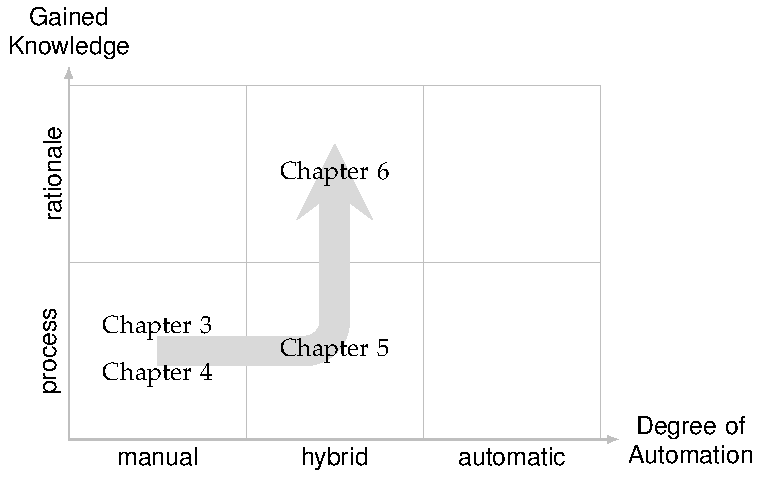
\includegraphics{work}
	\caption{Research problem split by \textcm{data} and \textch{task}. The horizontal axis represents different tasks and the vertical axis represents the complexity involved in the  task. The cells show the characteristics of data will be used to support the task.}
	\label{fig:intro-work}
\end{figure}

%\begin{enumerate}
%	\item time $\rightarrow$ temporal relationship
%	\item time + theme $\rightarrow$ complex temporal relationship
%	\item time $\rightarrow$ rational relationship
%	\item time + relation $\rightarrow$ complex rational relationship
%\end{enumerate}

We take a user-centered design approach in seeking solutions to all the research questions. For each question, we elicit the design requirements by conducting a user study and/or drawing from the literature. Visual encoding and interaction are designed to meet those requirements, and the designs are implemented into a working prototype. Finally, an empirical study is conducted to explore how the tool is used by target audience and check whether it provides the intended support. 

We aim to design general solutions that can be applied to sensemaking in various domains. However, as the solutions need to be empirically validated using target audience and real-world data, our implementation and evaluation focus on the two following domains. 

\begin{enumerate}
	\item \textbf{Intelligence analysis}. This is the domain where sensemaking was introduced into the visualization community with notable sensemaking models~\cite{Klein2003, Pirolli2005}.
	\item \textbf{Everyday, online sensemaking}. This hugely popular domain is how people usually make sense of their daily problems.
\end{enumerate}

\section{Thesis Contributions}
Toward the overall goal of supporting users in their sensemaking processes through the visualizations of provenance data, this thesis contributes:

\begin{itemize}
	\item A timeline visualization technique -- SchemaLine -- that enables users to examine information in chronological order, identify temporal patterns and construct narratives from relevant user annotations. SchemaLine produces a compact but aesthetically pleasing layout and a set of fluid interactions allowing users to perform various sensemaking activities described in the Data--Frame model~\cite{Klein2003}. This is to address Research Question 1.
	
	\item A timeline visualization technique -- TimeSets -- that enables users to explore complex temporal relationship by effectively representing both temporal and thematic provenance data. TimeSets visually groups data items that share the same theme but still preserves their temporal order. It colors the backgrounds of the entire themes to distinguish them and uses colored gradient backgrounds for the intersections among those themes. It also adjusts the level of details of each data item dynamically to accommodate more items within a given display estate. This is to address Research Question 2. 
	
	\item Qualitative research methods are often used in understanding rational relationship of sensemaking. This is a manual and time-consuming process: researchers collect observation data, transcribe screen capture videos and think-aloud recordings, identify recurring patterns, and eventually abstract the sensemaking process into a general model. We contribute a visual sensemaking tool -- SensePath -- that offers an alternative and possibly faster approach in performing transcription and coding. In stead of having to transcribe the video, SensePath automatically captures and detects participant's sensemaking actions, and provides multi-linked visualizations to support further analysis. It visualizes provenance data in a timeline that enables researchers to quickly gain an overview of the sensemaking process and identify recurring sensemaking patterns. It also links with a screen capture video to allow researchers to examine  additional context when necessary. Finally, to enable researchers to continue working on later stages of analysis using their normal workflow, SensePath exports its coded transcript in a common format that can be used by other popular qualitative data analysis software packages. This is to address Research Question 3.	
	
	\item A visual sensemaking tool -- SenseMap -- that enables users to explore and express complex rational relationship of sensemaking. It automatically captures and detects sensemaking actions and relationships between these actions before visualizing both of them in a branching history tree. This allows users to examine the rational relationship between the actions they performed and potentially helps them remind of what have been done earlier. SenseMap offers users to assign additional meaning to the automatically collected data by spatially grouping actions or adding rational links between them, in order to help explain complex relationship. Finally, SenseMap allow users to communicate their analysis results at different levels of granularity including a big picture of user-organized findings, a more detailed analysis process and raw provenance data captured. This is to address Research Question 4.
\end{itemize}

\section{Related Publications}

\subsection{Primary Publications} 
The following publications contain the core content presented in this thesis, from \autoref{chap:schemaline} to \autoref{chap:sensemap}.

\begin{itemize}
\item \textbf{P. H. Nguyen}, K. Xu, R.Walker, and B. L.W.Wong. SchemaLine: Timeline Visualization for Sensemaking. In \textit{International Conference on Information Visualization}, pages 225--233. IEEE, jul 2014.

This is the main content of \autoref{chap:schemaline}.

\item \textbf{P. H. Nguyen}, K. Xu, R. Walker, and B. L. W. Wong. TimeSets: Timeline visualization with set relations. \textit{Information Visualization}, 15(3):253--269, jul 2016. 

This is the main content of \autoref{chap:timesets}.

\item \textbf{P. H. Nguyen}, K. Xu, A. Wheat, B. L. W. Wong, S. Attfield, and B. Fields. SensePath: Understanding the Sensemaking Process through Analytic Provenance. \textit{IEEE Transactions on Visualization and Computer Graphics}, 22(1):41--50, jan 2016.

This is the main content of \autoref{chap:sensepath}.

\item \textbf{P. H. Nguyen}, K. Xu, A. Bardill, S. Betul, K. Herd, and B. L.W.Wong. SenseMap: Supporting Browser-based Online Sensemaking through Analytic Provenance. In \textit{IEEE Conference on Visual Analytics Science and Technology}, 2016.

This is the main content of \autoref{chap:sensemap}.
\end{itemize}

\subsection{Secondary Publications} 
The following publications also contribute to the ideas about provenance presented in this thesis.

\begin{itemize}
\item R. Walker, A. Slingsby, J. Dykes, K. Xu, J. Wood, \textbf{P. H. Nguyen}, D. Stephens, B. L. W. Wong, and Y. Zheng. An extensible framework for provenance in human terrain visual analytics. \textit{IEEE Transactions on Visualization and Computer Graphics}, 19(12):2139--2148, dec 2013.
\item K. Xu, S. Attfield, T. J. Jankun-Kelly, A. Wheat, \textbf{P. H. Nguyen}, and N. Selvaraj. Analytic provenance for sensemaking: a research agenda. IEEE Computer Graphics and Applications, 35(3):56--64, jan 2015.
\item K. Xu, \textbf{P. H. Nguyen}, and B. Fields. Visual analysis of streaming data with SAVI and SenseMAP. In \textit{IEEE Conference on Visual Analytics Science and Technology}, pages 389--390. IEEE, oct 2014.
\end{itemize}

\section{Thesis Outline} 
The remainder of this thesis is organized as follows.

First, \autoref{chap:review} reviews the core work related to sensemaking, analytic provenance and visualization. Then, it emphasizes on the visualization of provenance data for supporting sensemaking. At the end, this chapter presents visualization techniques of general time-oriented and network data because these types of data have similar characteristics as provenance data.

\autoref{chap:schemaline} discusses the SchemaLine timeline visualization of user annotations enabling the users to explore temporal relationship of sensemaking -- addressing Research Question 1.

\autoref{chap:timesets} extends \autoref{chap:schemaline} to present the TimeSets visualization technique that can effectively show both temporal and thematic provenance data in order to reveal complex temporal relationship of sensemaking -- addressing Research Question 2.

\autoref{chap:sensepath} discusses the SensePath visualization tool that can exploit time-oriented provenance data, enabling users to explore rational relationship of sensemaking -- addressing Research Question 3.

\autoref{chap:sensemap} describes the SenseMap visualization tool that can utilize both temporal and relational provenance data enabling users to explore and express complex rational relationship of sensemaking -- addressing Research Question 4.

Finally, \autoref{chap:conclusion} concludes the thesis with a discussion on its contributions and future research directions triggered from this work.